\chapter{Disturbances}
\section{Force loops}
	
	Whenever designing a precise system, an important key aspect to keep in mind is to decouple as much as possible measurements and side effects and in particular the forces.
	
	In fact there are no infinitely rigid material and so any force results in a displacement which can affect the measurement or precision when its magnitude is comparable with the resolution. Also we have to keep in mind that every mechanical system obey the Newton's first law and so we can recognize a balanced \textbf{loop of forces} acting within, and in particular we need to realize
	\begin{itemize}
		\item which forcer are related to the process performed by the system;
		\item what are the paths followed by those forces.
	\end{itemize}
	All force loops, due to the Newton's law, must be closed. Visualizing force loops helps in designing the structure and the interfaces, so that the process forcers  result in minimal deformations along all the force loop. In particular we have to consider that bearing (or in general element with lower elastic stiffness) subject to the force (due to the loop) doesn't deform with values out of the resolution range. In  general any deformation (in particular the one associated to thermal expansion due to temperature gradients that cannot be measured) along the loop directly produces a measurement error.
	
	\paragraph{Functional independence design principle} A good design tries to split functions into different subsystems and, to make their performances independent, so that one subsystem can be tuned/calibrated/adjusted independently without affecting the others.
	
	\paragraph{Metrology loop} A \de{metrology loop} is a structural loop of all elements whose dimensional changes would not be measure and the better is to have them as short as possible. With this said then it means that any mechanical play shall be kept out of it and be reduced.
	
	Often forces and metrology loops have different/incompatible requirements; as example a linear encoder (metrology loop) must be insensitive temperature (and so we can use INVER alloy) while the structure must be resistant and with high damping (and so cast iron is \textit{better}). This is another reason to apply the functional independence design principle and keep at minimum the interfaces between metrology and force (structural) loops; minimum interfaces often means (quasi-)kinematic mounts.
	
	\paragraph{Thermal loop} Path across an assembly of mechanical components which determines the relative position between specified objects under changing temperatures. Considering $L_s$ the length of components whose expansion relates to an expansion and and $L_c$ the one that close the loop, it means that
	\[ \Delta L = \sum_i L_{s,i} \alpha_i \, \Delta T_i - \sum _j L_{c,j} \alpha_j\, \Delta T_j \]
	This error can be compensated if we compute the temperatures of each part of the system (and in order to improve this we have to increase thermal conductivity to reduce thermal gradients). Another technique that can be used is to design symmetric structures that better rejects effects of thermal gradients with the drawback of having a larger, heavier, slower and more costly system.\\
	Using kinematic mounts two components can be made thermally invariant at one point known as \textbf{thermal center} (figure \ref{fig:dist:thermalcenter}).
	
	\begin{SCfigure}[2][bht]
		\centering 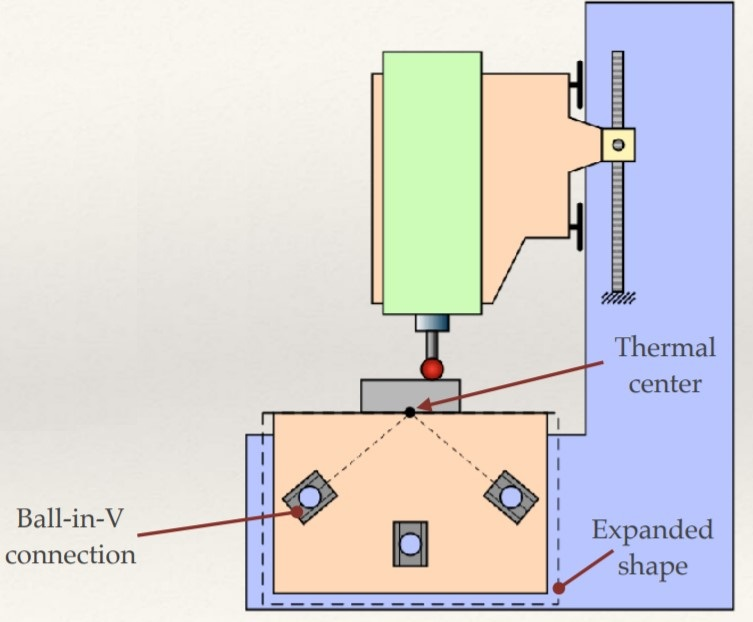
\includegraphics[width=6cm]{thermal-center}
		\caption{example of kinematic mount that allow to compensate temperature variation.} \label{fig:dist:thermalcenter}	
	\end{SCfigure}
	
	\paragraph{Maximum permissible error} Displacement and length precision measurement system declare their accuracy in form of \de{maximum permissible error}, a contractual figure to be verified upon first installation; there is no predefined methodology fo assessing this parameter and it's definition/calculation depends on the vendor and the manufacturer. In general it's not a good to choose a system over another based on the maximum permissible error declared  by the vendor.
	
	
\section{Materials selection}
	
	\de{Ashby maps} are 2D plot reporting pairs of related properties (like strength vs density) in $\log-\log$ plots reporting classes of materials as clouds (figure \ref{fig:dist:ashby}), making easier to understand which materials might suit for a certain application.
	
	\begin{figure}[bht]
		\centering 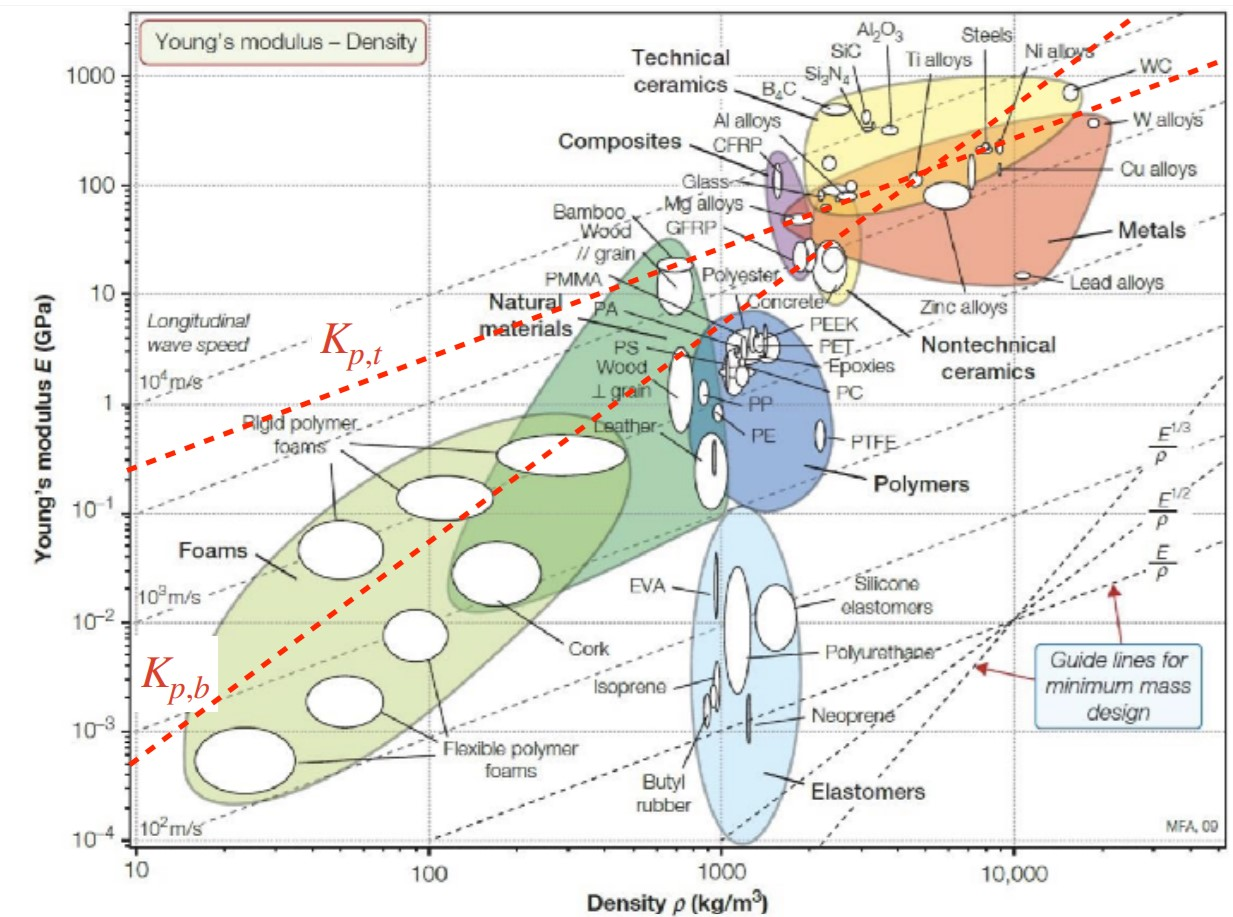
\includegraphics[width=11cm]{ashby}
		\caption{example of an Ashby map relating the density $\rho$ with the Young's module $E$ of different materials.} \label{fig:dist:ashby}
	\end{figure}
	
	\paragraph{Ashby performance index} In general, as example, a bar responds differently depending on the kind of load applied; considering a bar subjected to a pure tension load $P$, the stress state $\sigma$ and the weight $w$ can be evaluated as
	\[ \sigma = \frac P A \qquad \qquad w = \rho A L  \qquad \qquad \Rightarrow \quad w = \rho \frac P \sigma L = LP \frac \rho\sigma = \frac{LP}{K_{p,t}} \]
	In this relation the term $K_{p,t} = \sigma/\rho$ is the coefficient that relates material stiffness response (in a pure tension scenario) and it's mass $w$. Similarly if the bar is subjected to a pure bending moment $M$ we can define	
	\[ \sigma = -\frac {M}{I}y \qquad \qquad w = \rho A L  \qquad \qquad \Rightarrow \quad w = \sqrt{6MbL^2} \frac{\rho}{\sqrt{\sigma}} =  \frac{ \sqrt{6MbL^2}}{K_{p,b}}  \]
	In this case the coefficient $K_{p,b} = \sqrt \sigma/\rho$ refers to the coefficient that relates the material with equal mass to their stiffness response over the same bending moment. In figure \ref{fig:dist:ashby} is possible how the coefficient $K_{p,t}$ and $K_{p,b}$ can be used to determine materials that will result in same stiffness/mass behaviour.
	
	\paragraph{Chetwynd histograms} This kind of histograms (figure \ref{fig:dist:Chetwiynd}) reports different properties for two different materials: a bar going downward means that the first material is worst than the second (while if it's upward the response is better).
	
	\begin{SCfigure}[2][bht]
		\centering 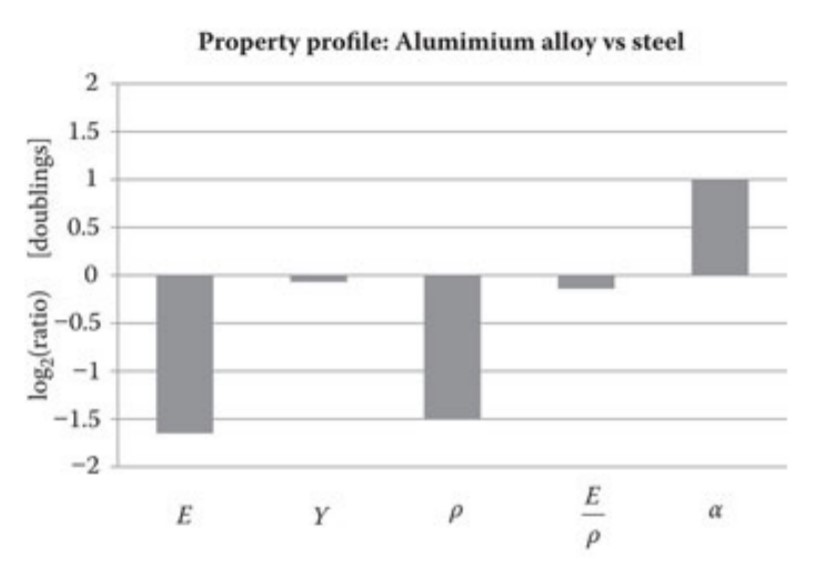
\includegraphics[width=6cm]{Chetwiynd}
		\caption{example of Chetwiynd histogram that compares aluminium alloys versus the steels one.} \label{fig:dist:Chetwiynd}	
	\end{SCfigure}
	
	In general vertical axis is logarithmic in order to focus on significant differences between materials. Properties, or \textbf{property groups}, are identified on the basis of selected use cases, factoring out any geometrical detail from the model.The underlying assumption is that, thanks to superposition of effects principle, the amount of change in behaviour by changing the material is not affected by the shape complexity.
	
	As example the tensile strength $\delta = \frac{Fl}{EA}$ of a bar relates only to the Young's module $E$ as property of the material,  and so can be evaluated in that property group. Another example is the maximum bending moment $M_{max}= \frac{2YI}{d}$ that's behave in the property group of the yielding strength $Y$. Also rational group properties can be defined like $\sqrt{E/\rho}$ that relates to the natural frequency of a beam. In general the typically considered property groups are
	\[ E \quad Y \quad \frac E \rho \quad \frac{\sqrt E}{\rho} \quad \frac{\sqrt[3] E}{\rho} \quad \frac Y E \quad \frac Y\rho \quad \frac k {cp} \quad \frac{cp}{\alpha} \quad \frac k\alpha \quad \frac k{\alpha E} \quad \frac 1 \alpha \quad \frac{1}{\alpha E} \]
	
	In general a way to pick the \textit{best} material for a specific application is to create a good-nut-not-excellent model material (that doesn't necessarily exists in real life) and confront him with a variety of real materials in order to find the one that suits most the application. As example figure \ref{fig:dist:chetcompr} compares a model material described in table \ref{tab:dist:modelmaterial} to spring steel.
	
	\begin{SCfigure}[2][bht]
		\centering 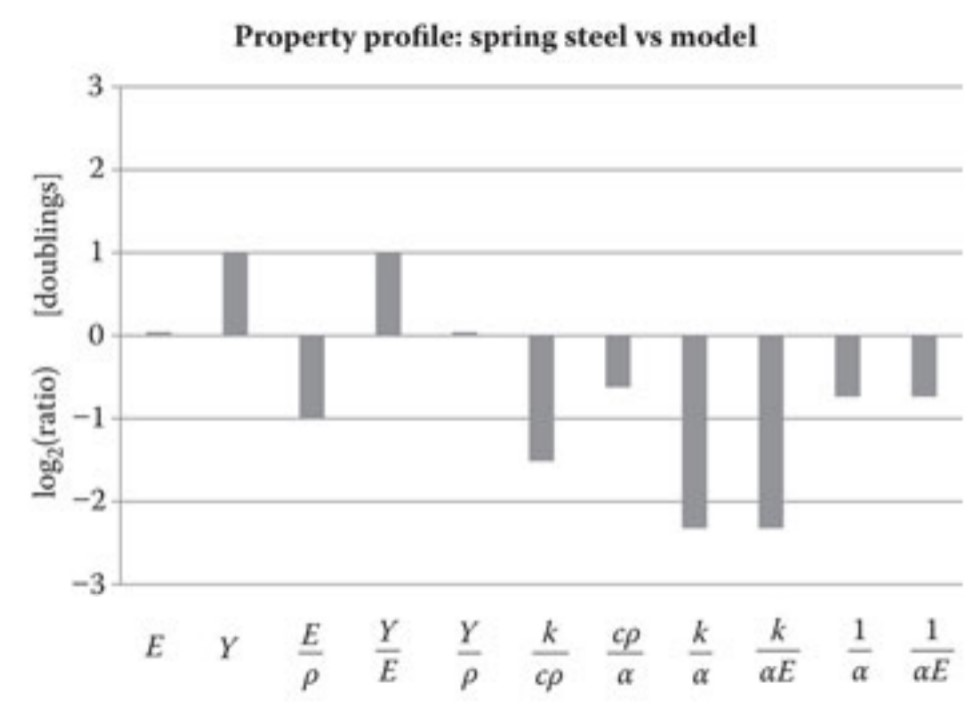
\includegraphics[width=6cm]{chet-model}
		\caption{example of Chetwynd histogram comparing spring steel and model material (table \ref{tab:dist:modelmaterial}).} \label{fig:dist:chetcompr}
	\end{SCfigure}
	
	\begin{table}[bht]
		\centering
		\caption{properties of the model material.} \label{tab:dist:modelmaterial}
		
		\begin{tabular}{r c | c | c }
			\textbf{Property} && \textbf{Typical of} & \textbf{Model value} \\ \hline
			modulus of elasticity & $E$ & mild steel & $200 GPa$ \\
			yield strength & $Y$ & mild steel & $300 MPa$ \\
			density & $\rho$ & oxide ceramic & $400 kg/m^3$ \\
			thermal expansion & $\alpha$ & oxide ceramic & $7\cdot 10^{-6} K^{-1}$ \\
			thermal conductivity & $k$ & Aluminum alloy & $150 W / m \, K$ \\
			specific heat & $c$ & many metals & $750 J / kg\, K$ \\
		\end{tabular}
		
	\end{table}
	
	
	\paragraph{Relevant metallic materials} For precise application the main materials are 
	\begin{itemize}
		\item steel: rather common due to availability, cost, ease of manufacture; it's an average performer;
		
		\item stainless steel: corrosion resistants and the non-magnetic property; usually the have worse performances and thermal property groups (compared to steel).
		
		\item cast iron: suitable for casting larger parts (such machine bases); it's pro's are the stability in time, the absorption of energy due to the graphite and the high damping coefficients;
		
		\item aluminum alloys: 2/3 times more costly than mild steel, similar to stainless steel, but lighter and with good thermal property groups (and so it's suitable for metrology loops  with lightly loaded structural loops);
		
		\item bronze and brass: were common precision materials due to their machinability and stability, while now are less common due to the technology improvement;
		
		\item tungsten: usually used as a thin film as buffer layer for accommodating thermal stresses;
		
		\item molybdenum: balanced perform respect to all metals;
		
		\item gold, platinum: thin layers or coatings to provide a particular surface layer functionality (such electrical, optical, electro-chemical, biocompatible ones);
		
		\item titanium alloys: marginally better than aluminum in mechanical property groups but word performer in thermal properties;
		
		\item INVAR (Iron, $36\%$ nickel alloy): similar to inox steels but with lower thermal expansion coefficient ($10$ times smaller).
	\end{itemize}
	
	
	
	
	
	
	
	
	
	
	
	
	
	
	
	


\section{Isolation}